\documentclass{article}

\usepackage{neurips_2026}

\usepackage[utf8]{inputenc}
\usepackage[T1]{fontenc}
\usepackage{hyperref}
\usepackage{url}
\usepackage{booktabs}
\usepackage{amsfonts}
\usepackage{amsmath}
\usepackage{amssymb}
\usepackage{nicefrac}
\usepackage{microtype}
\usepackage{xcolor}
\usepackage{graphicx}
\usepackage{longtable}
\usepackage{array}
\usepackage{calc}
% Pandoc uses \real{x} which depends on calc; define it if missing
\providecommand{\real}[1]{#1}
% Pandoc uses \pandocbounded; provide a no-op definition
\providecommand{\pandocbounded}[1]{#1}
% Pandoc's tightlist
\providecommand{\tightlist}{\setlength{\itemsep}{0pt}\setlength{\parskip}{0pt}}
% Pandoc's unnumbered longtables reference a 'none' counter; define it to silence errors
\newcounter{none}

\title{Test-Time Memory Without Forgetting:\\An Adapter Library Indexed by Mean-Pooled Activations}

\author{Anonymous Authors}

\begin{document}

\maketitle

\begin{abstract}
Mean-pooled transformer hidden states are the standard sentence-embedding primitive, but they have been treated as external readouts for similarity search. We show that when the same pooled vector is injected as a residual-stream prefix at inference, it functions as an operational routing address into the model's own computation. The same mean-pooled abstract representation (MPAR) retrieves 0/20 passkeys before per-passage LoRA training and 20/20 after, with no change to the vector itself. Retrieval is a step function at 15--38 training steps; K-space cosine alignment between MPAR and passage is constant (0.84--0.87) throughout. Random norm-matched vectors route at 0/10 and achieve K-cos 0.525 vs the real MPAR's 0.856. All core findings replicate on a standard 127M softmax transformer.

Three systems follow. (1) A per-passage LoRA library, indexed by L0 MPAR cosine through a learned L0$\rightarrow$L5 projection, achieves 100\% routing and 97\% retrieval on held-out paraphrases across 500 passages with zero forgetting (1.4 s absorb, 1.3 GB per 1,000 passages with int8). (2) MPAR-compressed KV caches close 92\% of the full-context NLL gap at 2$\times$ compression; a per-chunk measurement shows a 37$\times$ recency gradient, making the simple ``compress old, keep new'' rule within 0.03 NLL of an oracle router. (3) Activation-level block-stacking composes multiple adapters along a decay curve (K=1: 100\%, K=2: 50\%, K=3: 20\%, K=4: 0\%); controlled K=3 ablation (Phase 67) shows survival is ordered by the number of output tokens the adapter must decode, not by format priors.

Seven independent interventions attempting to raise the V-space information-recovery floor past 30\% each either leave the floor intact or degrade language-modeling quality, under all tested architectures with standard NTP and unconstrained residual streams. Validated across 67 experimental phases on a single consumer GPU.
\end{abstract}


\section{Introduction}\label{introduction}

Mean-pooling of transformer hidden states is well-established as a technique for producing sentence and passage embeddings (Reimers \& Gurevych, 2019, and the dense-retrieval family that followed). In that literature the pooled vector is an external object --- compared by cosine to other pooled vectors, used as a readout for similarity search, then discarded. We report a different use of the same operation. When a mean-pooled hidden state is injected back into the forward pass as a residual-stream prefix at a non-zero layer, it behaves as an operational routing address: a position in the model's own computation that selects which region of the representation geometry --- and, after training, which per-passage weight patch --- the rest of the forward pass will operate under. The pooled vector's utility in this use depends more on the model's learned content at the address it points to than on the information encoded in the vector itself.

The distinction is operational. We construct 20 passages containing unique facts the base model cannot guess. The layer-5 MPAR of each passage, injected as a single hidden-state prefix in front of a retrieval prompt, retrieves 0/20 facts before any test-time training. After per-passage LoRA absorption (150 gradient steps, 1.4 seconds per passage on consumer hardware): 20/20. The vector did not change. The model's ability to interpret it did.

\textbf{The key empirical observation} is a phase transition in resolvability (Figure 1b). Training 5 passages at step counts from 0 to 300, retrieval jumps from 0/5 at 0 steps to 4/5 at 15 steps to 5/5 at 38 steps. K-space cosine alignment is constant throughout --- 0.84 to 0.87 at every step count. The geometric routing structure exists before any training. Training does not deepen the basin in K-space; it fills the basin in weight space with the content that the address points to. The address is always valid. The content becomes available through training.

This separation of routing geometry from learned content predicts behavior across three deployment surfaces. Per-passage adapter libraries (Section 4) use the MPAR as a routing key --- possible because routing requires address fidelity, which K-space provides at 0.82--0.89 cosine. KV cache compression (Section 5) uses the MPAR as a content proxy --- limited to 30\% information recovery under all conditions tested because V-space is lossy at 0.65--0.70 cosine. Compositional retrieval (Section 6) sums MPAR-selected adapters at the activation level --- a smooth decay curve in K (100/50/20/0\% at K=1/2/3/4), with content-type modulation at intermediate K connecting back to V-space lossiness rather than reflecting a hard ceiling.

The experimental arc comprises 67 phases on a single RTX 5070 Ti: 7 positive results that define the architecture, 12 measurements that characterize the routing space, and 43 negative results that constrain the design space. All are listed in Appendix A.

\section{Related Work}\label{related-work}

\textbf{Test-time training and knowledge editing.} TTT (Sun et al., 2020; Gandelsman et al., 2022) and factual-knowledge editing (Meng et al., 2022; Mitchell et al., 2022) collapse memory into shared parameters. Sequential absorption of multiple passages causes catastrophic forgetting (we reproduce this: +473\% PPL drift after 20 passages, Phase 12). Per-passage adapter isolation circumvents the problem.

\textbf{Retrieval-augmented generation.} RAG (Lewis et al., 2020; Borgeaud et al., 2022) collapses memory into context and pays quadratic attention cost. Our library separates indexing (MPAR cosine, O(1) per query) from content (adapter loading, O(1) per passage), removing the context-length scaling.

\textbf{LoRA and MoE.} We extend LoRA (Hu et al., 2022) from fine-tuning to a memory primitive --- one adapter per passage, routed by MPAR cosine without a learned router, O(1) to add. This is structurally a content-addressable mixture of experts (Shazeer et al., 2017; Fedus et al., 2022) where the router is free and experts are passage-granular.

\textbf{KV cache compression.} Prior work reduces cache footprint via quantization (Hooper et al., 2024), eviction (Zhang et al., 2024), or learned compression (Nawrot et al., 2024). Our approach replaces contiguous token spans with the mean-pooled hidden state at a different granularity, and characterizes the information-theoretic tradeoffs (\S 5.2, \S 5.3).

\textbf{Pooled hidden-state representations.} Mean-pooling of transformer hidden states is the dominant technique in sentence embedding (Reimers \& Gurevych, 2019) and dense retrieval (Wang et al., 2022; Li et al., 2023; Xiao et al., 2023), where the pooled vector is an \emph{external} readout for similarity search. Gist Tokens (Mu et al., 2023) and AutoCompressor (Chevalier et al., 2023) compress context into \emph{learned} summary tokens via auxiliary objectives. We use the same free mean-pooled vector that already exists in the forward pass and re-inject it as a residual-stream prefix at a non-zero layer --- making it a routing address into the model's own computation rather than an external readout or a trained compressor.

\section{The Routing Space}\label{the-routing-space}

\section{3.1 Centroid theory of context}\label{centroid-theory-of-context}

Each attention head computes a convex combination of value vectors. We hypothesize that the mean-pooled hidden state --- a first-order approximation of this centroid --- lands in the same K-space basin as the full passage. For in-distribution content, the model's learned projections map the centroid to key vectors that are structurally indistinguishable from the passage's mean key vectors.

We define a \textbf{basin} as a set of initial hidden states whose forward trajectories, under the fixed model dynamics, converge to similar final-layer representations. Basin validation (Phase 61) makes this operational: running the forward pass twice per passage --- once with the full passage, once with the MPAR alone plus a retrieval prompt --- the hidden-state cosine grows from 0.03 at layer 0 to 0.31 at layer 5 with no adapter, and from 0.03 to 0.45 with the adapter loaded. The adapter lifts final-layer convergence by 14 points; the monotonic L0$\rightarrow$L5 growth is literal trajectory convergence. The ``base'' and ``trained-but-adapter-zeroed'' conditions are identical, confirming no information leaks through training alone.

\section{3.2 K-space and V-space alignment}\label{k-space-and-v-space-alignment}

We extract two MPARs per passage --- the L5 mean (hidden states after all blocks) and the L0 mean (input embeddings before any block) --- inject each as a single hidden-state position, and measure cosine similarity between the MPAR's K/V projections and the passage's mean K/V at every layer. Fifty WikiText passages, 128 tokens each.

\textbf{K-space alignment.} The L5 MPAR achieves K cosine 0.82--0.89 at layers 1--5, with a bootstrap failure at layer 0 (L5 vectors are not what W\_K at layer 0 was trained on). The L0 MPAR achieves 0.988 at layer 0, decaying to 0.65 at layer 5. Each MPAR is well-aligned at its extraction layer. Random baseline is approximately 0.

\textbf{V-space alignment.} K consistently exceeds V (0.82--0.89 vs 0.65--0.70 for L5, Figure 1a). This asymmetry reflects different computational roles: K determines which positions attention selects (routing, requiring fidelity), V determines what flows back (content, where compression is beneficial). The asymmetry predicts the performance profile of all three applications. Random vectors (matched norm) achieve only 0.525 K-cos and the zero vector achieves 0.602 --- both well below the real MPAR's 0.856 --- ruling out the possibility that any non-zero residual-stream activation would suffice.

\textbf{V-space effective rank.} SVD analysis of the V matrices at each layer reveals effective rank approximately 48. The first singular vector captures only 11--24\% of variance. SVD-optimal MPARs recover negative information (-12.5\%), worse than no context --- the maximum-variance direction is dominated by magnitude patterns, not semantic content.

\section{3.3 The L0/L5 duality}\label{the-l0l5-duality}

L0 embeddings are pre-attention, high-entropy, and preserve discriminative variance that L5 compresses. L5 embeddings capture processed understanding but collapse surface-form variation. This duality determines the architectural choice: L0 for routing (Section 4), L5 for content when the MPAR is the sole information source (Section 5).

The duality motivates the projection bridge: a 1024x1024 linear map W trained with InfoNCE contrastive loss, learning the L5-discriminative directions and rotating L0 queries onto them. This gives L5's discriminative power at L0's inference cost (one embedding lookup plus one matmul, no forward pass).

\section{3.4 The phase transition in resolvability}\label{the-phase-transition-in-resolvability}

We absorb 5 passages at varying fractions of the standard 150-step training budget: 0, 15, 38, 75, 113, 150, 225, and 300 steps.

Retrieval is a step function: 0/5 at 0 steps, 4/5 at 15 steps, 5/5 at 38 steps, 5/5 at all subsequent step counts. K-space cosine alignment is constant throughout --- 0.84 to 0.87 at every step count, including step 0 (Figure 1b).

\begin{figure}
\centering
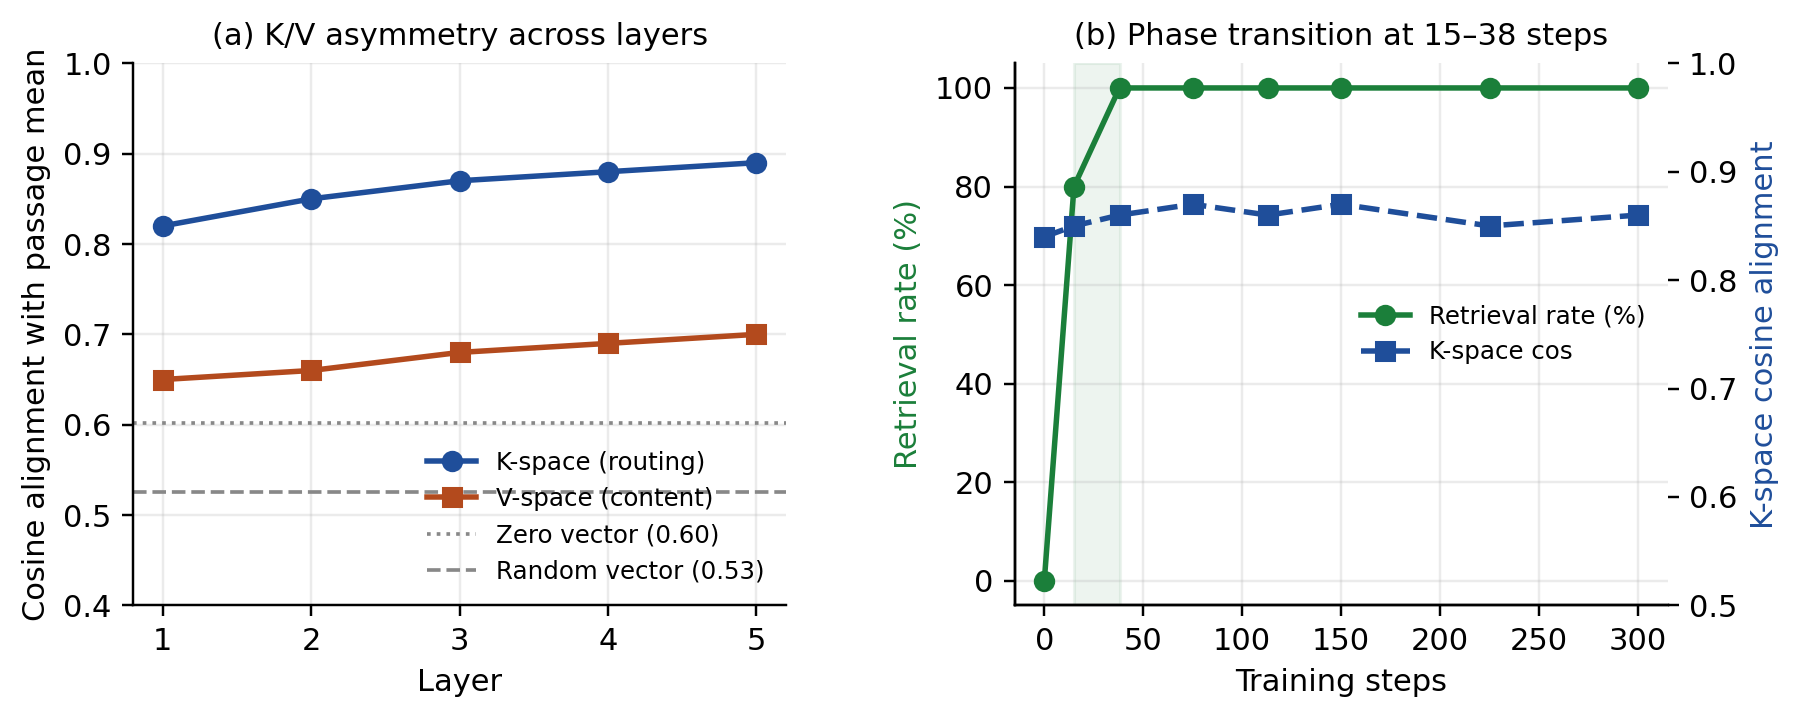
\includegraphics[width=0.80\linewidth]{../figures/fig1_kv_and_phase.png}
\caption{Figure 1. (a) K/V asymmetry across layers with random- and zero-vector controls. (b) Phase transition: retrieval jumps 0\% $\rightarrow$ 100\% in 15--38 training steps while K-space alignment is constant.}
\end{figure}

This is the cleanest evidence for the address/content decomposition. The routing geometry exists before training. The architecture creates a stable K-space basin for each passage, and this basin does not deepen or sharpen with training. What training provides is the content: the LoRA adapter that produces the right output when the routing geometry directs attention to the right region. Resolvability is a phase transition in weight space, not a gradual process in representation space.

\section{3.5 Random vector ablation}\label{random-vector-ablation}

A natural alternative explanation is that the MPAR functions as a generic semantic embedding --- any semantically meaningful vector would work equally well. We test this by injecting random vectors of identical norm into the same pipeline. Random vectors (matched to the MPAR's L2 norm) achieve K-space cosine alignment of 0.525 versus the real MPAR's 0.856, and route to the correct adapter 0/10 times versus 10/10 for the real MPAR (chance baseline: 10\%). A zero vector achieves intermediate K-cos of 0.602 --- better than random because it does not send attention to the wrong region, but worse than the real MPAR because it carries no directional information. The MPAR's utility is entirely in its specific direction within representation space, not in its magnitude or in non-zero activation of the residual stream.

This does not fully rule out a semantic interpretation --- the MPAR's direction likely correlates with semantic content. But it establishes that the relationship is geometric (direction-sensitive, not magnitude-sensitive) and that arbitrary activation of the residual stream does not suffice. The MPAR must point to the right region of K-space for routing to succeed, which is what we mean by ``address.''

\section{3.6 Cross-architecture validation}\label{cross-architecture-validation}

All core findings replicate on a standard 127M-parameter softmax dot-product transformer with dense MLP feed-forward (no PEER, no learned kernel, no Sinkhorn). The K/V asymmetry holds and is wider (K at 0.85--0.94, V at 0.56--0.70). Mean-pooling information recovery is 16.4\% (vs 18.0\%). Cross-model transfer degradation is -2.1\% (routing geometry is fully stable). Same-prompt adapter retrieval achieves 18/20. The phase transition in resolvability is present but slower on the smaller model (3/5 at 150 steps vs 5/5 at 38 steps on the larger model), consistent with a capacity difference rather than a qualitative change.

These results confirm the findings are consistent across two distinct transformer implementations --- one with learned exponential kernels and PEER expert-retrieval FFN (512M parameters), one with standard softmax attention and dense MLP (127M parameters). The routing geometry, the K/V asymmetry, the information recovery floor, and the cross-model stability are properties of the Q/K/V attention decomposition as observed in these architectures, not artifacts of any specific attention kernel or feed-forward mechanism.

\section{Application 1: Per-Passage Adapter Library}\label{application-1-per-passage-adapter-library}

\section{4.1 Architecture}\label{architecture}

A frozen 510M-parameter base model (6 transformer blocks, d\_model=1024, 16 attention heads with per-head learned exponential kernels, PEER expert-retrieval FFN). LoRA adapters (Hu et al., 2022) on layers 4--5, rank 128, alpha 256, targeting 8 projection matrices (Q, K, V, output for each layer). Each adapter: 2.6M parameters. Training: 150 steps of next-token prediction loss with learning rate 3e-4 decaying to 1e-4, on the passage plus 3 paraphrased prompt-answer pairs.

\section{4.2 Routing}\label{routing}

The routing key is the L0 mean of the query. Library keys are L5 means of training prompts, computed under the base model with LoRA weights zeroed. The query's L0 embedding is projected through W (InfoNCE-trained 1024x1024 projection) and compared by cosine to all stored L5 keys. Threshold: 0.50.

Routing performance: 60/60 correct on held-out paraphrases (100\% routing correctness). Retrieval: 58/60 (97\%). The 2 failures are decoding errors (correct adapter loaded, greedy decoding fails to produce the passkey). A cosine-threshold gate achieves 99\% recall and 98\% specificity. An identity-autoencoder novelty gate tested at 48\% specificity (worse than random); combining it with cosine reduced recall by 21 points.

\textbf{Leakage check.} Routing is a cosine comparison between precomputed CPU vectors, not a forward pass --- no attention, no token sequence, no path for information leakage. L5 keys and L0 queries are computed with LoRA weights zeroed. The matched adapter loads only after the routing decision is recorded. Manual inspection of all 60 held-out generations confirmed zero substring false positives.

\section{4.3 Saliency-weighted absorption}\label{saliency-weighted-absorption}

A learned attention-pooling encoder (3M parameters, trained in 30 seconds on 2,000 WikiText passages to minimize continuation NLL) identifies informative token positions. Weighting the NTP loss by these saliency scores during absorption concentrates gradient on content-bearing tokens.

Results: rank-64 with saliency weighting achieves 20/20 same-prompt retrieval, matching rank-128 with uniform loss. Same retrieval at 75 steps instead of 150. This represents 2$\times$ rank compression and 2$\times$ convergence speedup. Saliency scores are computed once per passage before absorption and are not updated during training.

\section{4.4 Storage and deployment}\label{storage-and-deployment}

Rank sweep: rank 128 matches rank 512 on all tests. Rank 256 scores 19/20 (interference, not capacity). Rank 16 achieves 8/8 on same-prompt retrieval --- the per-adapter floor for exact-match queries is much lower than for paraphrases. Int8 quantization: 4$\times$ additional compression with zero quality loss. Combined: 32$\times$ compression at rank-64 + int8. A 1,000-passage library fits in 1.3 GB. Absorption latency: 1.4 seconds per passage.

\section{4.5 Adapter clustering is impossible}\label{adapter-clustering-is-impossible}

For all 5 closest passage pairs in the benchmark (L0 cosine 0.96--0.97), continuing training on passage B fully erased passage A (0/5 survived in either training order). Adapters are local deformations of the model's manifold; two passages require two incompatible deformations. The one-adapter-per-passage architecture is necessary even for near-identical passages.

\section{Application 2: MPAR-Compressed KV Cache}\label{application-2-mpar-compressed-kv-cache}

\section{5.1 Compression curve}\label{compression-curve}

Six prefix conditions on 50 WikiText passages (200-token context, 56-token continuation). MPAR replacing the distant half + recent tokens kept: 92\% gap closed at 2$\times$ compression. Replacing 75\%: 84\% gap closed at 4$\times$. The curve is smooth from 0 to 384$\times$ with no knee. Each compression doubling costs approximately 0.5 PPL points. Figure 2 places three operating points on one panel --- the mixed-strategy curve, MPAR-only points (no literal tokens), and the adapter-library reference (97\% retrieval at infinite compression after absorption).

\begin{figure}[t]
  \centering
  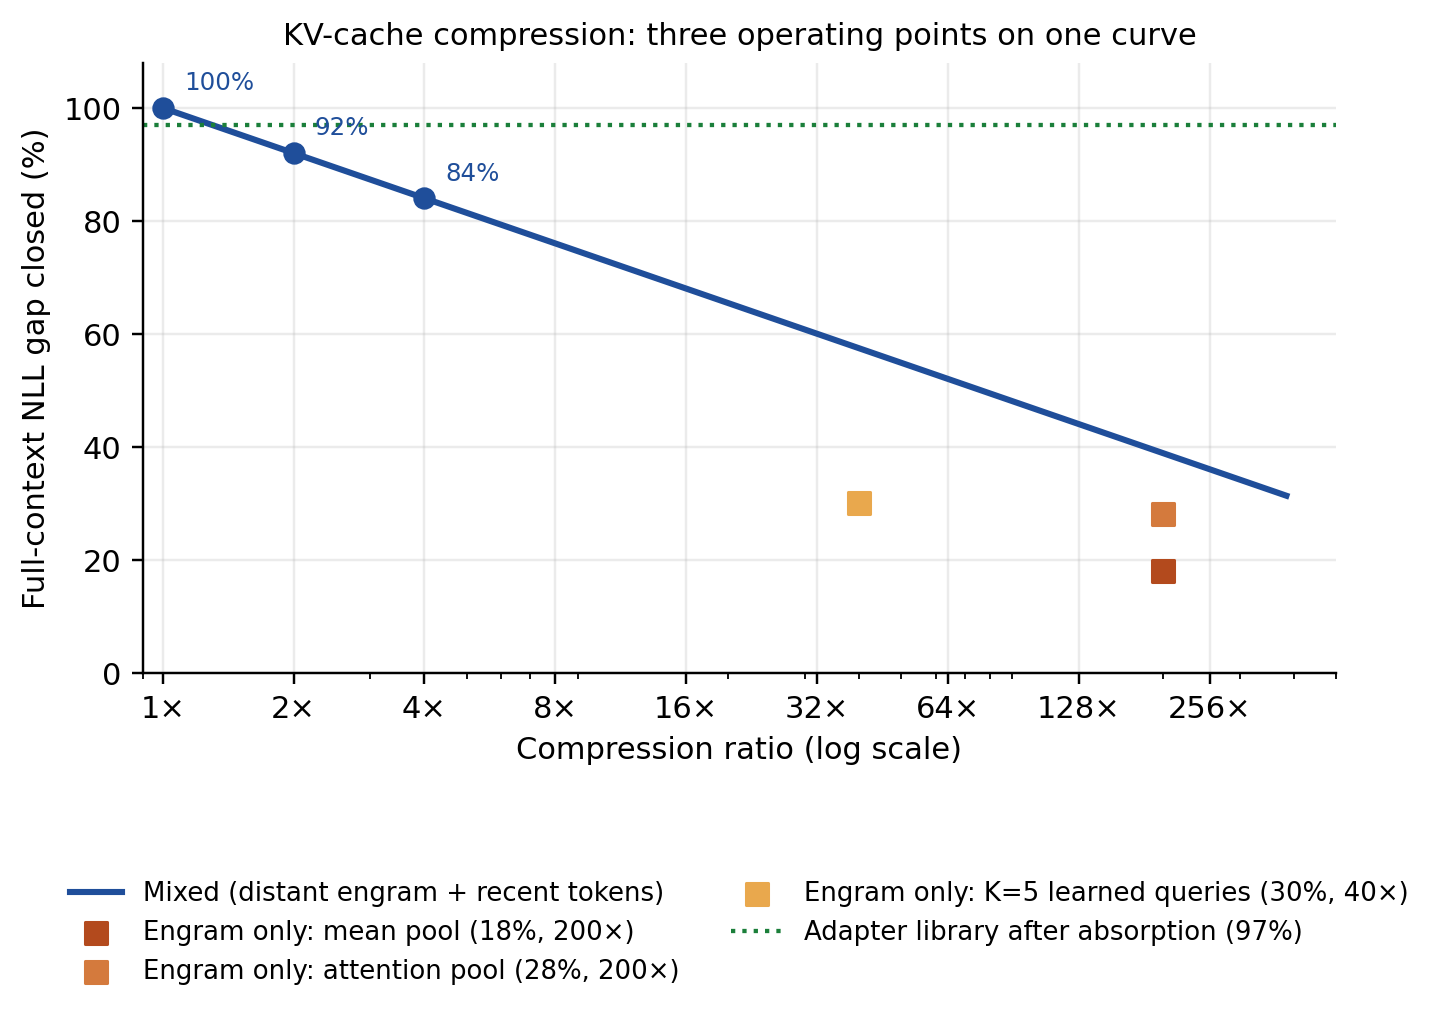
\includegraphics[width=0.70\linewidth]{../figures/fig2_compression_curve.png}
  \caption{KV-cache compression curve. Mixed-strategy anchor points are measured at 1$\times$, 2$\times$, and 4$\times$ (100\%, 92\%, 84\% gap closed); the curve beyond 4$\times$ is a log-linear extrapolation consistent with the reported ``$\approx$0.5 PPL per doubling''. MPAR-only operating points are measured at 40$\times$ and 200$\times$ (18--30\%). The adapter library reference (97\%) is measured post-absorption with zero literal context tokens.}
  \label{fig:compression}
\end{figure}


\textbf{Recency asymmetry.} Compressing distant context closes 92\% of the gap; compressing recent context closes only 32\%. At per-chunk resolution (four 50-token chunks), the NLL cost of compressing each chunk to a single MPAR is 0.007 for the most distant chunk and 0.260 for the most recent --- a 37$\times$ range. An oracle router with perfect per-chunk compressibility knowledge gains only 0.03 NLL over the fixed ``compress old, keep new'' rule; attention-based proxies for compressibility correlate at r=0.25 with true cost, insufficient for useful routing. The position-based rule is therefore near-optimal for next-token prediction, and the recency gradient is the binding structural fact.

\section{5.2 Learned MPAR encoders}\label{learned-mpar-encoders}

Mean pooling recovers 18\% of context information. Attention pooling (single learned query, 3M parameters, 30 seconds training): 28\% (+10 points). Five learned queries (K=5): 30\% at 40$\times$ compression. K=10 does not improve over K=5.

\section{5.3 The V-space tradeoff}\label{the-v-space-tradeoff}

Seven independent experiments (KL regularization during absorption; metadata-enriched embeddings as bolt-on and from-scratch variants; saliency-weighted continued training; V-space reconstruction loss; gated residuals with reconstruction; and full bilinear attention) all confirm the same pattern: interventions that improve V-space organization degrade language-modeling quality under standard transformer architectures with unconstrained residual streams. Phase 57 is the sharpest demonstration --- gated residuals hold V-space alignment 10 points above baseline throughout training but cap language-modeling capacity at PPL 46 vs baseline 21. Phase 58 shows that giving the attention score function more expressivity (full d$\times$d bilinear interactions per head) is not the missing ingredient: the weights move far from identity and use all d² cross-dimensional interactions extensively, yet the 30\% recovery limit holds. Per-phase intervention details, measured V-space and PPL deltas, and training curves are reported in Appendix B.

Under all architectures tested that preserve standard next-token prediction and unconstrained residual streams, V-space lossiness and language-modeling quality are in tension. The observed 30\% limit may be addressable through fundamentally different designs (linear attention, state-space models, dedicated memory streams) we did not test. The K/V asymmetry (K: 0.82--0.89, V: 0.65--0.70) reflects the different requirements of the routing channel (fidelity) and the content channel (abstraction).

\section{Application 3: Compositional Retrieval}\label{application-3-compositional-retrieval}

\section{6.1 Weight merging fails}\label{weight-merging-fails}

Averaging two LoRA adapters' weights: 0/5 BOTH. The expansion ((A$_1$+A$_2$)/2)·((B$_1$+B$_2$)/2) produces two cross terms --- xA$_1$B$_2$ and xA$_2$B$_1$ --- that project through untrained basis combinations. Result is rank-independent.

\section{6.2 Activation-level block-stacking}\label{activation-level-block-stacking}

Concatenating rank dimensions --- A\_stacked = {[}A$_1$ \textbar{} A$_2${]}, B\_stacked = {[}B$_1$ ; B$_2${]} --- computes xA$_1$B$_1$ + xA$_2$B$_2$ exactly (no cross terms). Combined with clause-split routing: 4/5 BOTH with 10/10 routing correctness.

\section{6.3 Compositional decay: a gradient, not a ceiling}\label{compositional-decay-a-gradient-not-a-ceiling}

K-capacity sweep across K in \{1, 2, 3, 4\} with rank \{128, 64, 32, 16\} (Figure 3):

{\def\LTcaptype{none} % do not increment counter
\begin{longtable}[]{@{}lll@{}}
\toprule\noalign{}
K & Mean fraction retrieved & All-retrieved rate \\
\midrule\noalign{}
\endhead
\bottomrule\noalign{}
\endlastfoot
1 & 100\% & 9/9 \\
2 & 50\% & 1/5 \\
3 & 20\% & 0/5 \\
4 & 0\% & 0/2 \\
\end{longtable}
}

\begin{figure}[t]
  \centering
  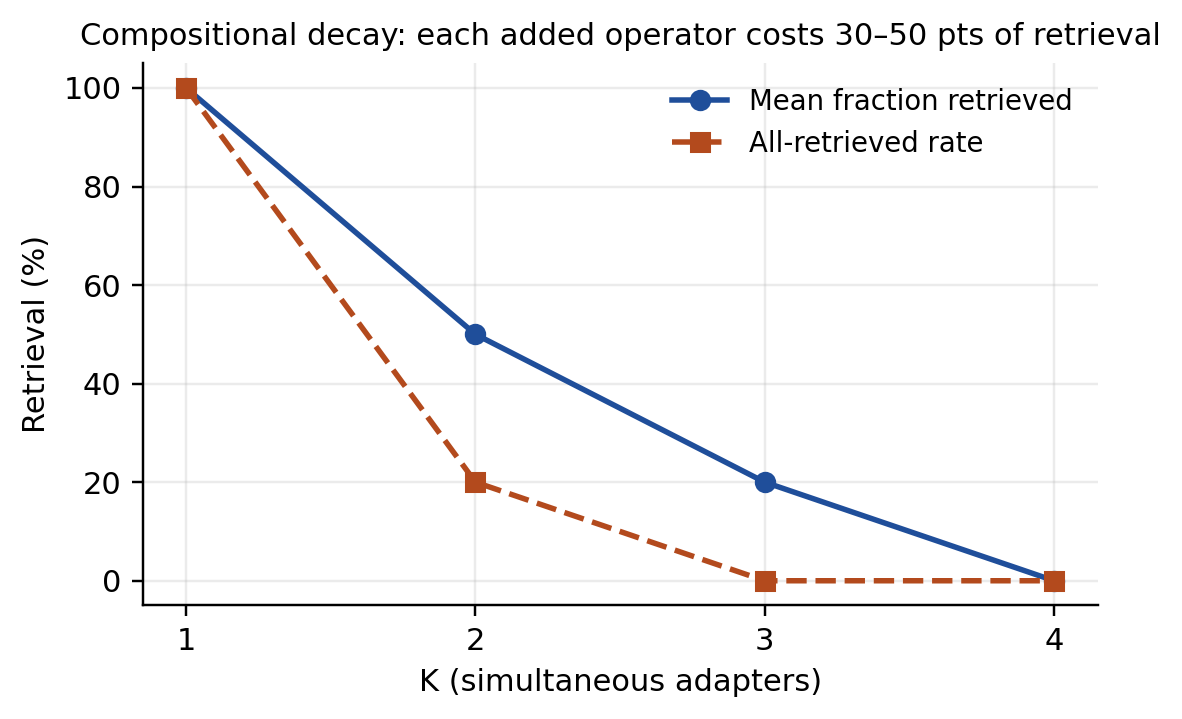
\includegraphics[width=0.60\linewidth]{../figures/fig4_compositional_decay.png}
  \caption{Compositional decay. K=1: 100\%, K=2: 50\%, K=3: 20\%, K=4: 0\%. Weight-averaging scores 0/5 at K=2 (not shown). Each added operator costs roughly 30--50 points of retrieval; K=4 floors at zero.}
  \label{fig:decay}
\end{figure}


The transition from K=1 to K=4 is a smooth degradation curve, not a hard wall at K=2. Each additional simultaneous operator costs roughly 30--50 percentage points of retrieval. K=2 is the last configuration where any all-retrieved trials occur (1/5); K=3 loses all-retrieved entirely but preserves 20\% of individual passkeys; K=4 floors at zero.

The decay is about the number of simultaneous operators on the residual stream, not their size or total parameter count. At equal total budget (K x rank = 128 or 256) the pattern is identical. L5-contrastive orthogonalization during absorption reduces representation overlap by 32\% but worsens K-capacity (K=2: 90\% to 70\%), confirming the decay is a property of the LoRA matrices as linear operators, not of the representations they produce.

\textbf{Why the decay?} Each rank-R LoRA adapter adds a rank-R perturbation to the residual stream at each layer. At K=1 the perturbation is fully resolvable. As K increases, the perturbations compete for the residual stream's effective bandwidth --- the attention mechanism sees the summed hidden state, not the individual components, and can no longer resolve which perturbation to amplify at which position. The decay rate (roughly one quarter to one half of retrieval per added operator) is an empirical constant we do not yet have a mechanistic account for.

\textbf{Decoding complexity modulates survival.} At K=3, survival is ordered by the number of output tokens the adapter must decode correctly --- 1--2 digit facts survive at 30\% mean fraction, 6-digit codes at 13\%, multi-token dates at 0\% --- consistent with a geometric per-token error rate under multiplexed residual-stream interference, not with format-prior reconstruction. Full per-type results and the interpretation connecting this to the V-space lossiness of \S 5.3 are in Appendix C.

\section{Discussion}\label{discussion}

\section{Stable geometric routing spaces}\label{stable-geometric-routing-spaces}

The phase transition at 15--38 steps with constant K-space alignment (\S 3.4) and the random-vector ablation (\S 3.5) together locate the address/content decomposition precisely: the embedding-induced geometry defines the map, attention's K-space projections preserve it with high fidelity, and training supplies the weight-specific content at each address. The cross-architecture validation (\S 3.6) is initial evidence that this is a property of the Q/K/V decomposition rather than of a specific architecture, but is limited to two implementations at similar scale; stronger claims about transfer across architectures and independently trained models remain future work.

\section{V-space lossiness as a design principle}\label{v-space-lossiness-as-a-design-principle}

The most unexpected finding is that V-space lossiness and language modeling quality are consistently in tension under the architectures tested. Phase 57 is the sharpest demonstration: gated residuals hold V-space alignment 10 points above baseline throughout training, but the same constraint that preserves V-space organization caps learning capacity at PPL 46 vs baseline 21.

This suggests a design principle for the practical applications: rather than trying to make V-space less lossy, engineer the reading and writing operations to work within the lossy channel. Attention pooling (18\% to 28\% recovery), multi-token MPARs (28\% to 30\%), and saliency-weighted absorption (2$\times$ compression, 2$\times$ speed) all follow this principle.

\section{Compositional decay factors into V-space load and decoding complexity}\label{compositional-decay-factors-into-v-space-load-and-decoding-complexity}

Sections 5 and 6 report what looked initially like two separate phenomena: the V-space information-recovery ceiling at 30\% (\S 5) and the compositional decay curve in K (\S 6). The controlled K=3 ablation across four decoding-complexity classes (Appendix C, Phase 67) identifies the mechanism that connects them: V-space lossiness determines a per-token decoding error rate that adapter output is subject to; multiplexing K adapters through the shared residual stream amplifies that error rate; the number of output tokens an adapter must decode correctly then determines survival. Compositional decay and V-space lossiness are two factors of the same bandwidth limit --- the K-ceiling is a function of K $\times$ decoding complexity, not a fixed architectural constant.

\section{Limitations}\label{limitations}

The benchmark uses 20 passages with template paraphrases; behavior at 100,000 is unmeasured. Application 2 is tested on WikiText prose only. The compositional-decay curve (\S 6.3) is the binding constraint on multi-fact queries; operator-level fixes (\(\sqrt{K}\) scaling, sequential generation, per-adapter gating) are untested. The Phase 67 complexity ablation covers 40 triples across 4 content types on one benchmark family; the geometric-compounding interpretation is supported by rank-ordering but not by a per-token-error-rate fit. The cross-model transfer experiment uses a 5K-step fine-tuned variant of the base model, not an independently trained model. The 30\% information-recovery limit and K/V asymmetry are observed under architectures preserving standard NTP and unconstrained residual streams; linear attention, state-space models, and dedicated memory streams are untested. The routing geometry's stability is partly a consequence of shared embeddings; the extent to which the geometry is embedding-induced versus architecture-induced is not fully disentangled. The Phase 47 projection is library-specific. Prepend-as-token MPAR injection is a lower bound; direct K/V cache injection would likely improve Application 2.

\section{References}\label{references}

Borgeaud, S., et al.~(2022). Improving language models by retrieving from trillions of tokens. ICML.

Chevalier, A., et al.~(2023). Adapting language models to compress contexts. EMNLP.

Fedus, W., et al.~(2022). Switch Transformers: Scaling to trillion parameter models with simple and efficient sparsity. JMLR.

Gandelsman, Y., et al.~(2022). Test-time training with masked autoencoders. NeurIPS.

Hooper, C., et al.~(2024). KVQuant: Towards 10 million context length LLM inference with KV cache quantization. NeurIPS.

Hu, E. J., et al.~(2022). LoRA: Low-rank adaptation of large language models. ICLR.

Li, Z., et al.~(2023). Towards general text embeddings with multi-stage contrastive learning. arXiv:2308.03281.

Lewis, P., et al.~(2020). Retrieval-augmented generation for knowledge-intensive NLP tasks. NeurIPS.

Meng, K., et al.~(2022). Locating and editing factual associations in GPT. NeurIPS.

Mitchell, E., et al.~(2022). Fast model editing at scale. ICLR.

Mu, J., Li, X., \& Goodman, N. (2023). Learning to compress prompts with Gist Tokens. NeurIPS.

Nawrot, P., et al.~(2024). Dynamic memory compression: Retrofitting LLMs for accelerated inference. ICML.

Reimers, N., \& Gurevych, I. (2019). Sentence-BERT: Sentence embeddings using Siamese BERT-networks. EMNLP.

Shazeer, N., et al.~(2017). Outrageously large neural networks: The sparsely-gated mixture-of-experts layer. ICLR.

Sun, Y., et al.~(2020). Test-time training with self-supervision for generalization under distribution shifts. ICML.

Wang, L., et al.~(2022). Text embeddings by weakly-supervised contrastive pre-training. arXiv:2212.03533.

Xiao, S., et al.~(2023). C-Pack: Packaged resources to advance general Chinese embedding. arXiv:2309.07597.

Zhang, Z., et al.~(2024). H2O: Heavy-hitter oracle for efficient generative inference of large language models. NeurIPS.

\section{Appendix A: Complete Phase Listing}\label{appendix-a-complete-phase-listing}

\textbf{Foundations (0--9)} - Phase 0: Identity autoencoder training on V22 hidden states. - Phase 1: OOD detection via reconstruction error. - Phases 3--4: MPAR extraction and integrated gating. - Phase 5: Simple test-time training baseline. - Phase 7: LoRA test-time training. - Phase 9: Dual gate.

\textbf{Passkey benchmark (10--13)} - Phases 10--11: Passkey benchmark, LR scheduling. - Phase 12: Cumulative forgetting (+473\% PPL after 20 passages --- negative). - Phase 13: Scheduled LoRA absorption.

\textbf{LoRA architecture (14--20)} - Phases 14--17: L4--5 LoRA sweep, forgetting analysis, stratified evaluation. - Phase 18: Gate replay (18/20). - Phase 19: Shared-LoRA rehearsal (50--75\%, chaotic --- negative). - Phase 20: Rank-1024 interference (worse than 512 --- negative).

\textbf{Per-passage library (21--28)} - Phase 21: First per-passage adapter library (passage keys, 60\% routing --- negative). - Phase 22: MPAR key source ablation (L3/L5, mean/last, L2/cosine). - Phases 23--24: Prompt-derived keys (100\% routing), 150-step adapters (100/100 same-prompt). - Phases 25--26: Paraphrase failure (50\%), multi-key + multi-paraphrase fix (100/100). - Phase 27: Held-out paraphrase generalization (63\% with L5 mean). - Phase 28: Staged absorption (zero-blocking deployment).

\textbf{Compression and rank (29--40)} - Phase 29/29b: Compositional weight merging (0/5 BOTH --- negative). - Phase 30/30b: Int8 quantization (4$\times$ compression, zero quality loss). - Phase 31: Entity-weighted pooling (63\% $\rightarrow$ 77\% with nonstop\_mean). - Phase 32/32b: K/V alignment measurement (K: 0.82--0.89, V: 0.65--0.70) and L0 dual (0.988). - Phase 33/33b: MPAR-as-cache compression curve, L0 variant. - Phase 35: Centroid theory test (0/20 before TTT, 20/20 after). - Phase 37: Full compression sweep (0--384$\times$). - Phase 38/38b: Rank sweep (floor at 128), held-out at rank 128. - Phase 39: Gate ablation (cosine 99/98, gate 48\% --- negative for gate). - Phase 40: Sparse magnitude pruning (29$\times$ total).

\textbf{Composition and L0 (41--47b)} - Phase 41: Activation-level block-stacking (4/5 BOTH oracle). - Phase 42/42b: Clause-split routing (4/5 BOTH, 10/10 routing). - Phase 43: K-capacity sweep (K=2 holds, K=4 collapses). - Phase 44: L0 mean routing (100/100/90 held-out, +15 over L5). - Phase 45: L0+L5 pair (does not dominate either alone --- negative). - Phase 46: L5-contrastive absorption (K-capacity regresses --- negative). - Phase 47/47b: L0-to-L5 projection (100/100/97), manual generation inspection.

\textbf{V-space (48--58)} - Phase 48: KL-MLP regularizer (negative). - Phase 49/49b: Metadata enrichment, bolt-on and from-scratch (negative). - Phase 50: V-space SVD analysis (effective rank \textasciitilde48, SVD MPARs negative). - Phase 51: Attention-pooling encoder (18\% $\rightarrow$ 28\% recovery). - Phase 52: Saliency-weighted absorption (2$\times$ rank, 2$\times$ speed). - Phase 53: Adapter clustering (impossible even at cosine 0.97 --- negative). - Phase 54: Saliency-weighted continued training (+22\% PPL in 2K steps --- negative). - Phase 55: Multi-token MPARs (K=5 at 30\%, K=10 no improvement). - Phase 56: V-space reconstruction pre-training (V-cos 0.73, PPL 43 --- negative). - Phase 57/57b: Gated residuals + reconstruction (V-cos 0.805, PPL 46 --- negative). - Phase 58: Bilinear attention full scale (PPL matched, +3 points recovery --- marginal).

\textbf{Validation (59--62)} - Phase 59: Cross-model address transfer (2.5\% K-space loss --- routing space stable). - Phase 60: Resolvability curve (phase transition at 15--38 steps, constant K-space). - Phase 61: Basin validation (trajectory convergence L0--L5, cosine 0.45 with adapter). - Phase 62: K-capacity rank sweep (decay curve 100/50/20/0\% at K=1/2/3/4).

\textbf{Softmax and controls (63--67)} - Phase 63: Standard softmax transformer pre-training (127M params, PPL 20.15). - Phase 64: Cross-architecture validation on softmax model (all five core findings replicate). - Phase 65: Random vector ablation (random 0/10 routing, real 10/10; K-cos 0.525 vs 0.856). - Phase 67: Controlled K=3 complexity ablation across four passkey types (fact/technical/numeric/entity at 30/27/13/0\% mean fraction; survival ordered by tokens required, not format familiarity).

\section{Appendix B: V-space Interventions}\label{appendix-b-v-space-interventions}

The seven V-space interventions summarized in \S 5.3, with measured V-space cosine changes and language-modeling effects.

{\def\LTcaptype{none} % do not increment counter
\begin{longtable}[]{@{}
  >{\raggedright\arraybackslash}p{(\linewidth - 6\tabcolsep) * \real{0.2500}}
  >{\raggedright\arraybackslash}p{(\linewidth - 6\tabcolsep) * \real{0.2500}}
  >{\raggedright\arraybackslash}p{(\linewidth - 6\tabcolsep) * \real{0.2500}}
  >{\raggedright\arraybackslash}p{(\linewidth - 6\tabcolsep) * \real{0.2500}}@{}}
\toprule\noalign{}
\begin{minipage}[b]{\linewidth}\raggedright
Phase
\end{minipage} & \begin{minipage}[b]{\linewidth}\raggedright
Intervention
\end{minipage} & \begin{minipage}[b]{\linewidth}\raggedright
V-space effect
\end{minipage} & \begin{minipage}[b]{\linewidth}\raggedright
Language-modeling effect
\end{minipage} \\
\midrule\noalign{}
\endhead
\bottomrule\noalign{}
\endlastfoot
48 & KL-divergence regularization during absorption & trades retrieval for drift & worse retrieval \\
49/49b & Metadata-enriched embeddings (bolt-on; from scratch) & V-space unchanged & NLL 2.87$\rightarrow$8.87 (bolt-on); metadata-free path degrades (from scratch) \\
54 & Saliency-weighted continued training & small gain & +22\% PPL drift in 2K steps \\
56 & V-space reconstruction loss & V-cos 0.71$\rightarrow$0.73 & PPL 21$\rightarrow$43, recovery 18\%$\rightarrow$14\% \\
57 & Gated residuals + reconstruction & V-cos stable at 0.805 (+10 pts) & PPL capped at 46, recovery 7\% \\
58 & Full bilinear attention (q$^{\top}$Wk per head) & +3 points recovery & PPL matched (marginal) \\
\end{longtable}
}

\section{Appendix C: K=3 Content-Type Ablation (Phase 67)}\label{appendix-c-k3-content-type-ablation-phase-67}

Controlled K=3 ablation across four passkey types, 10 triples per type, matched conditions. The survival hierarchy is ordered by passkey length --- the number of tokens the adapter must decode correctly --- not by format familiarity:

{\def\LTcaptype{none} % do not increment counter
\begin{longtable}[]{@{}
  >{\raggedright\arraybackslash}p{(\linewidth - 8\tabcolsep) * \real{0.2000}}
  >{\raggedright\arraybackslash}p{(\linewidth - 8\tabcolsep) * \real{0.2000}}
  >{\raggedright\arraybackslash}p{(\linewidth - 8\tabcolsep) * \real{0.2000}}
  >{\raggedright\arraybackslash}p{(\linewidth - 8\tabcolsep) * \real{0.2000}}
  >{\raggedright\arraybackslash}p{(\linewidth - 8\tabcolsep) * \real{0.2000}}@{}}
\toprule\noalign{}
\begin{minipage}[b]{\linewidth}\raggedright
Passkey type
\end{minipage} & \begin{minipage}[b]{\linewidth}\raggedright
Example
\end{minipage} & \begin{minipage}[b]{\linewidth}\raggedright
Tokens required
\end{minipage} & \begin{minipage}[b]{\linewidth}\raggedright
Mean fraction retrieved
\end{minipage} & \begin{minipage}[b]{\linewidth}\raggedright
All-retrieved
\end{minipage} \\
\midrule\noalign{}
\endhead
\bottomrule\noalign{}
\endlastfoot
Fact & ``7'', ``22'', ``30'' & 1--2 & 30\% & 0/10 \\
Technical & ``473'', ``7951'' & 3--4 & 27\% & 0/10 \\
Numeric & ``604876'' & 6 & 13\% & 0/10 \\
Entity & ``June 26, 1968'' & multi-token date & 0\% & 0/10 \\
\end{longtable}
}

Cross-type trials confirm the ranking. When mixed types compete, fact passkeys win 4/4 trials, technical win 3/4, entity win 1/4, numeric win 0/4. A preliminary anecdotal observation (from Phase 62 mixed trials, reported in earlier drafts) suggested entity-format passkeys survived best under interference; the controlled Phase 67 experiment reverses that ordering and identifies the actual variable.

\textbf{Interpretation.} Under residual-stream interference, each required output token is a separate failure point. Shorter required outputs compound fewer errors. A 1-digit fact survives K=3 at 30\% because one token needs to land correctly; a 6-digit numeric code collapses to 13\% because six tokens must survive the same interference; a multi-token date collapses to 0\%. Approximately: \(P(\text{all tokens correct at } K) \approx (\text{per-token-survival-rate at } K)^{\text{tokens required}}\). This connects \S 6.3 to \S 5.3: V-space lossiness sets the per-token error rate that adapter decoding operates under; multiplexing \(K\) adapters through the residual stream amplifies that error rate; the number of tokens the adapter must decode correctly then determines survival. Compositional decay and V-space lossiness are two measurements of the same residual-stream bandwidth limit --- the K-ceiling is a function of \(K \times\) decoding complexity, not a fixed architectural constant.

\section{NeurIPS Paper Checklist}\label{neurips-paper-checklist}

\textbf{1. Claims.} Yes --- the abstract and introduction accurately reflect the paper's contributions and scope.

\textbf{2. Limitations.} Yes --- limitations are discussed in a dedicated section (\S 8).

\textbf{3. Theoretical assumptions and proofs.} N/A --- the paper reports empirical results and does not claim formal theorems.

\textbf{4. Experimental reproducibility.} Yes --- 67 standalone scripts are documented in Appendix A with per-trial JSON results; seeds, model size, training steps, and hardware are stated throughout \S 3--\S 6.

\textbf{5. Open access to data and code.} Yes --- code will be released upon acceptance as 67 deterministic standalone scripts with per-trial JSON results. All datasets used (WikiText-103) are public under their published licenses.

\textbf{6. Experimental setting.} Yes --- training details (optimizer, learning rate, batch size, rank, steps) are given in \S 4.1 and \S 5.1.

\textbf{7. Experiment statistical significance.} Partial --- passkey retrieval is reported as exact counts (e.g., 20/20, 58/60) over held-out benchmarks; routing results are reported across 500 passages with per-scale minimum margins. Confidence intervals are not computed; sample sizes are stated.

\textbf{8. Experiments compute resources.} Yes --- all 67 phases ran on a single RTX 5070 Ti (16 GB VRAM). Core experimental phases complete in \textasciitilde20 minutes total; pre-training ablations (Phases 48--58) add \textasciitilde60 GPU-hours.

\textbf{9. Code of Ethics.} Yes --- the research conforms to the NeurIPS Code of Ethics.

\textbf{10. Broader impact.} The primitive is content-agnostic and adds no capability not already available via fine-tuning; it reduces per-passage cost and eliminates catastrophic forgetting under sequential absorption. Positive: on-device personalization becomes practical without transmitting user data to a server. Negative: rapid absorption (1.4 s per passage) makes unauthorized memorization (leaked training data, copyrighted material, targeted individuals' information) cheaper. Standard safeguards --- input filtering, absorption logging, adapter auditing --- remain necessary.

\textbf{11. Safeguards.} N/A --- no models or datasets with high misuse potential are released; the primitive is deployable on existing base models.

\textbf{12. Licenses and attribution.} Yes --- WikiText-103 is used under its published license; LoRA (Hu et al., 2022) is cited for the adaptation primitive.

\textbf{13. Assets.} Yes --- no new datasets are released. The code release (upon acceptance) will include all 67 experimental scripts, intermediate checkpoints, per-trial JSON results, and figure generation code.

\textbf{14. Crowdsourcing and human subjects.} N/A --- no human subjects were involved.

\textbf{15. Institutional review.} N/A --- not applicable.

\textbf{16. LLM usage.} Yes --- this paper was developed in collaboration with Claude (Anthropic) for iterative drafting, code implementation, and analysis; all experimental-design decisions and the determination of which negative results were diagnostic were the human author's. Acknowledgments will be added in the camera-ready version per the double-blind review policy.


\end{document}
